%!TEX root = main.tex

\chapter{Estado del arte}
El proyecto Bio2RDF utiliza las tecnologías de la web semántica para su
implementación y funcionamiento. Así, el análisis que se hará en esta memoria
toma estos conocimientos como base y generará a través de ellos estadísticas de
centralidad con las cuales se determinará cuales son los datos más importantes
del \emph{dataset}.

Para poder analizar el problema correctamente es necesario el conocimiento de
las tecnologías que se enuncian en este capítulo. En la sección \ref{ea:ws} se
describe qué es la web semántica y las tecnologías que la componen.
En la sección \ref{ea:bio} se hace una revisión al proyecto Bio2RDF y en la
sección \ref{ea:cent} se introduce el concepto de centralidad junto a sus
métricas y algoritmos.
%TODO

\section{Web Semántica}\label{ea:ws}
La web semántica es un conjunto de actividades propuestas por la \emph{World
Wide Web Consortium} (desde ahora W3C) con el objetivo de generar tecnologías
para la publicación de datos en la web de tal manera que sean procesables por
las maquinas. 
Se basa en la idea de añadir metadatos semánticos y ontológicos que describan el
contenido y la relación entre los datos publicados. De esta manera se logra
mejorar la interoperatividad de internet pues los programas podrán acceder a los
datos en un lenguaje formal, procesar su contenido, razonar en base a este y
combinarlo para resolver problemas cotidianos automáticamente.

Es posible rastrear los orígenes de esta idea hasta una propuesta temprana de la
\emph{world wide web} en 1986 ~\cite{berners1989proposal} y el subsecuente
trabajo de Berners-Lee et al.\cite{berners1992world} donde se prevé la
necesidad de una evolución desde objetos legible por las personas a información
semántica orientada a las máquinas.

Para lograr los objetivos de la web semántica se han generado múltiples
metalenguajes y estándares de representación como son XML, XML Schema, RDF,
RDF Schema, OWL y SPARQL. Estas tecnologías se utilizan actualmente para generar
datos enlazados (\emph{Linked Data}), que buscan enlazar información arbitraria
en la web generando así una ``red de las cosas del mundo, descrita por los datos
en la Web'' \cite{berners2011linked}.

\begin{figure}[htpb]
  \centering
  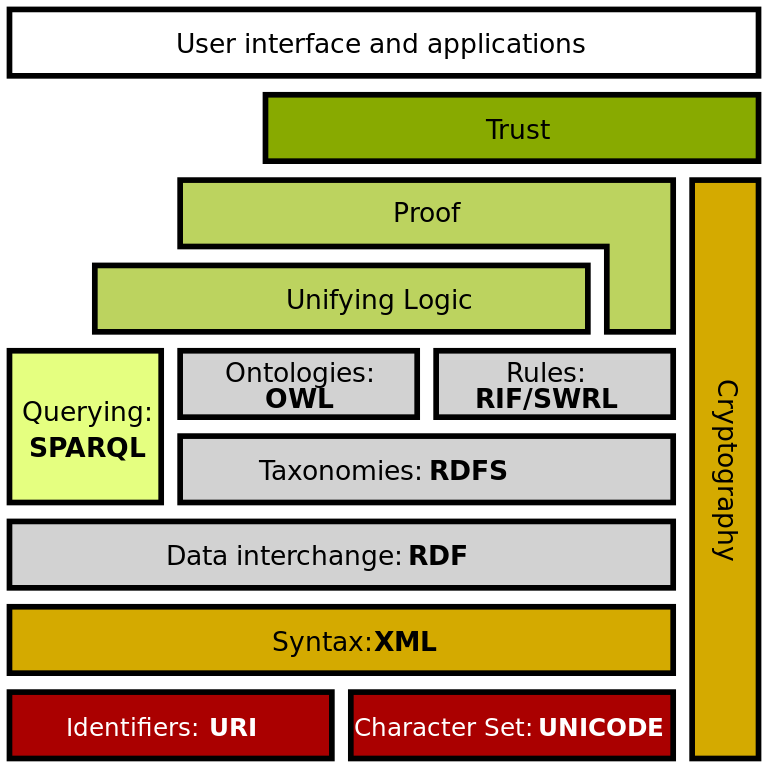
\includegraphics[width=.6\textwidth]{figures/Semantic_web_stack.png}
  \caption{Pila de tecnologías de la web semántica.}
  \vspace{-.25cm}
  \caption*{Creado por Marobi1\cite{wikimg:swstack}.}
  \label{fig:swstack}
\end{figure}

En las siguientes secciones se describirán más detalladamente algunos de los
conceptos presentados en la figura \ref{fig:swstack} comenzando desde la base,
con las tecnologías del hipertexto (URI y XML), para luego pasar a las
tecnologías de la web semántica más estandarizadas (RDF, RDFS y OWL) y terminar
con el lenguaje de consulta SPARQL.

\subsection{URI}
Una URI (del las siglas del ingles \emph{Uniform Resource Identifier}) es una
cadena de caracteres utilizada para identificar un recurso inequívocamente.
Si bien en un principio solo acepta un subconjunto caracteres ASCII (el alfabeto
en ingles y los números) y código porciento (por ejemplo '\%26' es '\&') el
estándar fue extendido el 2005 a IRI (\emph{Internationalized resource
identifier}) que puede contener caracteres Unicode/ISO 10646, incluyendo chino,
japones, koreano, entre otros\cite{gangemi2006bourne}. En este documento no se
diferenciará entre URI y IRI.

La sintaxis actual de una URI fue definida por Berners-Lee et al. el
2005 ~\cite{berners2004uniform} como sigue:\\
\texttt{
  scheme:{[//{[user:password@]}host{[:port]}]}{[/]}path{[?query]}{[\#fragment]}
}\\
donde:
\begin{itemize}
  \item
    El \bf{esquema} (\emph{scheme}) que consiste en una secuencia de caracteres
    sensibles a las mayúsculas que comienza con una letra y es seguido por
    cualquier combinación de letras, puntos (\tt{.}), guiones (\tt{-}) y signos
    más (\tt{+}), terminando con dos puntos (\tt{:}). 
    Ejemplos populares son \tt{http}, \tt{ftp} y \tt{mailto}.
  \item
    Las dos barras (\tt{//}) son requeridos para algunos esquemas. Cuando la
    componente de autoridad no está presente la ruta no puede comenzar con dos
    barras.
  \item
    La \bf{autoridad} se divide como sigue:
    \begin{itemize}
      \item
        Una \bf{autentificación} opcional compuesta por el usuario
        (\emph{user}), dos puntos y una contraseña (\emph{password}) terminando
        en un arroba (\tt{@}).
      \item
        Un anfitrión (\emph{host}) que puede ser un nombre registrado un una
        dirección IP.
      \item
        Un número de \bf{puerto} opcional (\emph{port}) separado del anfitrión
        por dos puntos.
    \end{itemize}
  \item
    Una \bf{ruta} (\emph{path}) que es una secuencia de segmentos separados
    por una barra (\tt{/}) que comienza con una de las mismas. Generalmente
    representa la localización de un archivo en un sistema de archivos
    jerárquico pero no es necesario.
  \item
    Una \bf{consulta} opcional (\emph{query}) que comienza con un signo de
    interrogación (\tt{?}) y, a pesar de no tener un sintaxis claramente
    definida, usualmente presenta pares atributo-valor.
  \item
    Un \bf{fragmento} opcional (\emph{fragment}) que comienza con un numeral
    (\tt{\#}) seguido por un identificador secundario al recurso principal.
\end{itemize}

\begin{figure}[htpb]
  $$
    \underbrace{\text{http}}_{\text{esquema}}\text{://}
    \overbrace{
      \overbrace{
        \underbrace{\text{user:password}}_{\text{autentificación}}\text{@}
        \underbrace{\text{example.com}}_{\text{anfitrión}}\text{:}
        \underbrace{\text{80}}_{\text{puerto}}
      }^{\text{autoridad}}
      \overbrace{\text{/path/data}}^{\text{ruta}}
    }^{\text{parte jerárquica}}\text{?}
    \underbrace{\text{key=value}}_{\text{consulta}}\text{\#}
    \underbrace{\text{section1}}_{\text{fragmento}}
  $$
  \caption{Ejemplo de una URI.}
  \label{fig:uriex}
\end{figure}

Un ejemplo de lo anterior sería la figura \ref{fig:uriex} donde podemos notar
que una URL (\emph{Uniform Resource Locator}) es una URI, pero no debemos
confundir los términos pues una URL además de identificar un recurso web permite
obtener una representación del mismo generalmente en formato HTML vía HTTP. Es
decir, una URL es una URI que apunta a un recurso físico en la web, mientras que
una URI no necesariamente debe apuntar a una localización que exista realmente.

\subsection{XML}
XML es la abreviación del ingles \emph{Extensible Markup Language} es un
lenguaje de marcas desarrollado por el W3C para almacenar datos de manera
legible tanto por personas como por máquinas. 
El diseño de XML busca la simplicidad, generalidad y usabilidad a través de
internet\cite{paoli2004extensible}. 

Un documento XML puede comenzar con un identificador declarando alguna
información sobre el documento en sí. Luego el cuerpo del fichero debe contener
solo un elemento raíz y dentro de éste se pueden escribir múltiples elementos y
atributos.

\begin{figure}[htpb]
  \centering
  \begin{tabular}{c}
    \lstinputlisting[
      basicstyle=\ttfamily\scriptsize,
      language=xml]{Codigo/example-xml.xml}
  \end{tabular}
  \caption{Ejemplo de XML.}
  \vspace{-.25cm}
  \label{fig:xmlex}
\end{figure}

En la figura \ref{fig:xmlex} vemos la libertad que nos da XML a la hora de
representar cualquier tipo de información, pero esta libertad hace que
interpretar la validez de un documento sea complicado, pues la información
contenida en este puede ser sensible a la aplicación y el lenguaje definido con
esta tecnología. En respuesta a esta problemática la W3C desarrolló \emph{XML
Schema} que cobra vital importancia para la web semántica.


\subsection{XSD}
XSD (del ingles \emph{XML Schema Definition}) es una recomendación del W3C que
especifica formalmente la estructura y restricciones de los contenidos de un
fichero XML de manera precisa más allá de las normas sintácticas del propio
lenguaje XML.

A diferencia de otros lenguajes de esquemas para XML, XSD especifica también
tipos de datos y sus restricciones, logrando un estándar a la hora de
representar datos básicos \cite{biron2004xml}. 
Presenta 19 tipos de datos básicos: \tt{anyURI},
\tt{base64Binary}, \tt{boolean}, \tt{date}, \tt{dateTime}, \tt{decimal},
\tt{double}, \tt{duration}, \tt{float}, \tt{hexBinary}, \tt{gDay}, \tt{gMonth},
\tt{gMonthDay}, \tt{gYear}, \tt{gYearMonth}, \tt{NOTATION}, \tt{QName},
\tt{string} y \tt{time}. Además permite la creación de nuevos tipos de datos por
medio de tres mecanismos:
\begin{itemize}
  \item \bf{Restricción:} Reduce los valores que puede tomar un dato.
  \item \bf{Lista:} Permite una secuencia de valores.
  \item \bf{Unión:} Permite la elección de valores de diferentes tipos.
\end{itemize}

Gracias a estos factores un fichero XML Schema puede representar un modelo de
datos completo y robusto, con relaciones entre los datos y tipos de datos
básicos. Esta característica es fundamental para la web semántica.

\begin{figure}[htpb]
  \centering
  \begin{tabular}{c}
    \lstinputlisting[
      basicstyle=\ttfamily\scriptsize,
      language=xml]{Codigo/example-xmls.xml}
  \end{tabular}
  \caption{Ejemplo de XMLS.}
  \vspace{-.25cm}
  \caption*{Definiendo una película con XSD.}
  \label{fig:xsdex}
\end{figure}

\subsection{RDF}
\subsection{RDFS}
\subsection{SPARQL}

\section{Proyecto Bio2RDF}\label{ea:bio}
\section{Métricas de centralidad}\label{ea:cent}

%\section{Algoritmos de acceso eficiente a grafos}
%\subsection{Algoritmos de búsqueda en grafos}
%\subsection{Vecinos más cercanos}
%\subsection{Relaciones entre nodos de grafos}
